\chapter{Conclusions}

\section{Gateway Locations}

% Evaluate the chosen gateway locations and give example of the ranges, etc.
% Also add graphs of recorded gateway ranges from TTN Mapper?
This section will evaluate the chosen gateway locations as described in \cref{sec:gateway-locations} and give some examples of the ranges that can be achieved with them.
The maps used to show range data were taken from the \emph{Advanced Maps} feature of \ac{TTNM}.
Thus, as explained in \cref{subsec:cleaning-collected-data}, they may contain some inaccuracies and outliers.

\subsection{\acf{GHB} student dormitory}\label{subsec:ghb-student-dormitory-range-results}

The MikroTik gateway deployed on top of the \ac{GHB} student dormitory is the gateway with the highest range in Furtwangen.
This doesn't come as a surprise, given its exposed location on top of a hill plus the height of the building itself.

\begin{figure}
    \centering
    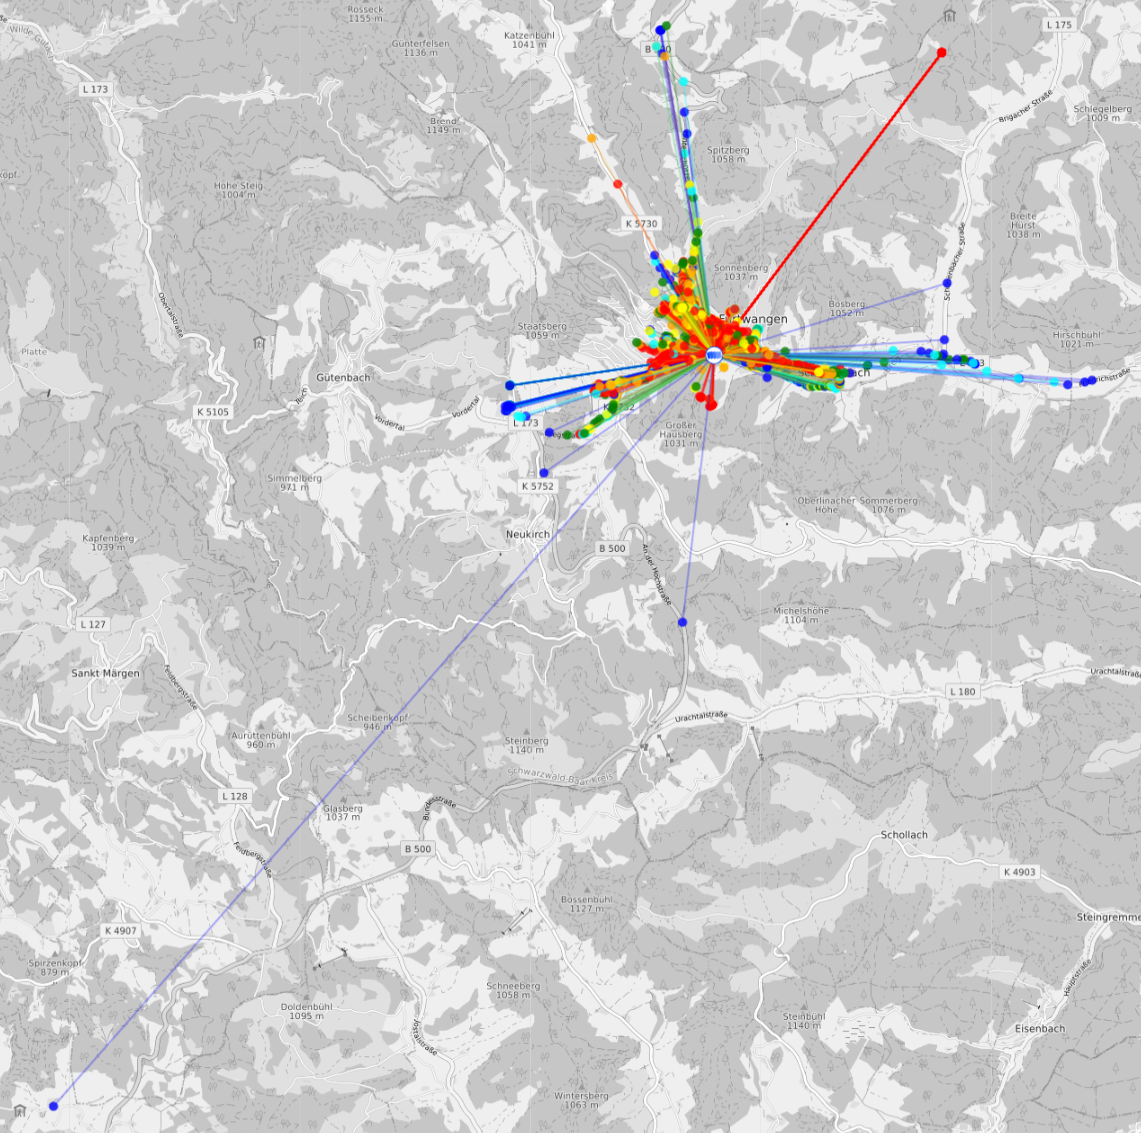
\includegraphics[width=1\textwidth]{pictures/ttn-mapper/gateway-ranges/ghb_mikrotik_gw_range.png}
    \caption{
        Map of some \ac{TTNM} data points taken from the \ac{LoRaWAN} gateway deployed on top of the \ac{GHB} student dormitory.
        The data point on the lower left is the maximum range recorded for this gateway --- \SI{14.2}{\kilo\meter}.
        However, it can be considered an outlier, as the next highest range is \SI{5.3}{\kilo\meter} away from the gateway (on the far right).
    }\label{pic:ghb_mikrotik_gw_range}
\end{figure}

The maximum range recorded for this gateway is \SI{14.2}{\kilo\meter}, which is the blue point in the lower left-hand corner of \cref{pic:ghb_mikrotik_gw_range}.
While that data point may be considered an error or outlier, a more realistic one is the blue point on the rightmost side of the image which is \SI{5.3}{\kilo\meter} away from the gateway.

\subsection{\ac{HFU} C building}

When viewed alongside the results from the \ac{GHB} gateway shown in \cref{subsec:ghb-student-dormitory-range-results}, the results from the \ac{HFU} C building gateway are exactly as one would expect.
Since the Antenna was the same MikroTik one as the one used with the \ac{GHB} gateway, the coverage behavior is similar.
The ranges as a whole are slightly lower which stems from the fact that the \ac{HFU} C building is located inside the Bregtal valley and thus has a lower elevation than the \ac{GHB} student dormitory.

\begin{figure}
    \centering
    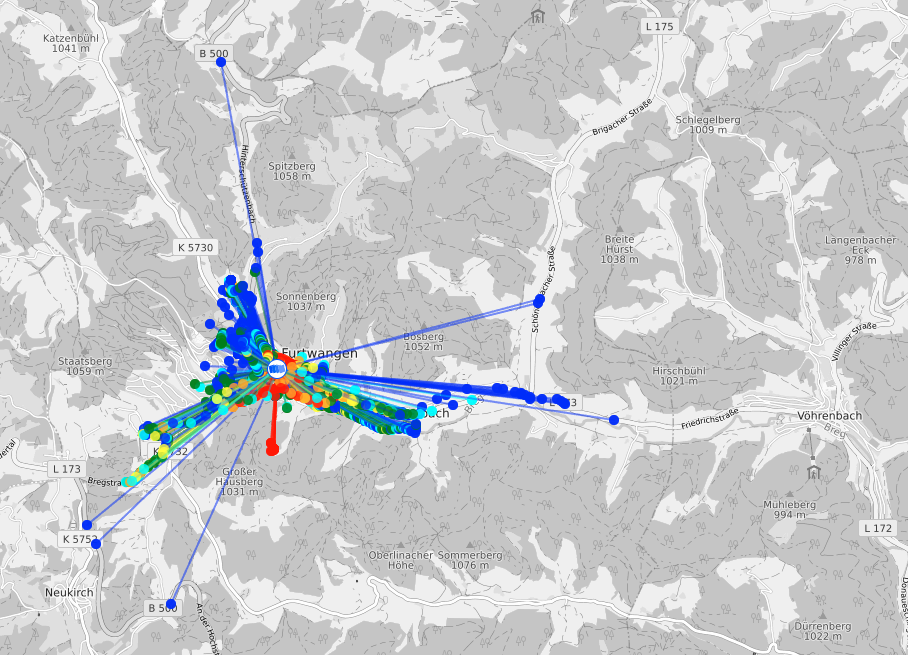
\includegraphics[width=1\textwidth]{pictures/ttn-mapper/gateway-ranges/c_building_gw_range.png}
    \caption{
        Map of some \ac{TTNM} data points taken from the \ac{LoRaWAN} gateway deployed on top of the C building.
        The slightly smaller range compared to \cref{pic:ghb_mikrotik_gw_range} is evident.
        The maximum range, however, is still \SI{4.3}{\kilo\meter} which is the rightmost blue point in the direction of Vöhrenbach.
    }\label{pic:c_building_gw_range}
\end{figure}

\Cref{pic:c_building_gw_range} shows the range of the \ac{HFU} C building gateway.
Clearly visible is the slightly smaller range compared to \cref{pic:ghb_mikrotik_gw_range}.
The maximum range recorded for this gateway is \SI{4.3}{\kilo\meter}, which is the rightmost blue point in the direction of Vöhrenbach again.

\subsection{\acf{ASH}}

% TODO

\subsection{\emph{DL0FIS} amateur radio club station}

% TODO

\section{Collected data in Furtwangen on \acl{TTNM}}\label{sec:collected-data-in-furtwangen-on-ttnm}

% TODO: add before and after images of TTN Mapper heatmap

% TODO mention that collecting sats and accuracy data also would have been possible

\subsection{\acl{TTNM} heatmap view after additional data collection}\label{sec:ttm_heatmap_after}

% TODO add after image of TTN Mapper heatmap

\section{Comparison of Geolocation Methods}

% TODO compare the geolocation methods

\subsection{\acf{RSSI}}

% TODO: mention the problems with RSSI-based geolocation (different antennas per gateway, different antennas per node, different environments, etc.)

\subsection{\acf{ToA} / \acf{TDoA}}

% TODO: not feasible due to lack of nanosecond level timestamps as well as the fact that the gateways' timestamps are not synchronized with the nodes' timestamps in all cases

\subsection{Fingerprinting}

% TODO: describe how this worked and how it could be improved (worked pretty okay but has only limited accuracy)

% TODO: mention the potential of using machine learning to improve the fingerprinting method

\section{Comparison of findings with existing work}

% TODO mention the existing work in conjunction with my own findings as far as localization is concerned

\section{Problems}

% Mention problems with falsely entered gateway locations and how they could be fixed

% TODO write some more about this
As mentioned in \cref{sec:spreading-factors}, using a different \ac{SF} on the end devices can also impact the accuracy of the geolocation methods because they influence the \ac{RSSI} values.

\section{Outlook}

% TODO: What else can be done? What are the next steps?

\subsection{Shortcomings of the \acf{TTNL} software}

% TODO: show what else could be done - automatically recognize if gateways moved too far away like in TTN Mapper etc.

\subsubsection{Automatically detecting moved gateways}

\subsubsection{Remove dependency on \acl{TTNM}}

% TODO: Mention how own REST endpoints similar to TTN Mapper could be used to get the data without having to rely on TTN Mapper

\subsection{Projects made possible due to new \acs{LoRaWAN} gateways in Furtwangen}

% TODO: is this necessary?

As there are now several new \ac{LoRaWAN} gateways in Furtwangen, there are several projects that can be done in the future that would not have been possible before without installing such gateways by oneself.

This section will list some of these projects and describe how they could be implemented.

\subsubsection{Measuring the water level of the Breg river}

One of the \ac{LoRaWAN} nodes ordered as part of this thesis is a \emph{Milesight EM310-UDL}, an ultrasonic distance/level sensor.
As the \ac{LoRaWAN} network coverage of Furtwangen is now adequate, it would be possible to use this sensor to measure the water level of the Breg river flowing through the vicinity of the \ac{HFU}.
This would allow for a more accurate prediction of the water level of the Breg river, which might in turn allow for a more accurate prediction of the water level of the Danube river.
Installing this \ac{LoRaWAN} node as well as connecting it to \ac{TTN} and adding an \acf{AS} to it to allow monitoring of the water level of the Breg river would be a good future project for students of the \ac{HFU}, enabled by the gateways placed during this thesis.

\subsubsection{Measuring soil moisture and environmental conditions in the Furtwangen city park}

This same semester, Samuel Kasper, a student of the \ac{DM} faculty of the \ac{HFU} wrote his bachelor thesis about measuring the humidity as well as the temperature of the soil to monitor plants and crop growth.
The installation of \ac{LoRaWAN} gateways in the city of Furtwangen helped him in this regard, as he did not have to install his own gateways and instead could use the now existing infrastructure in the city.

\subsubsection{Monitoring of Gateways}

Another possible project would be an application that monitors the gateways and checks if they are still online.
Such a project could be realized with software like \emph{Node-RED}.

\subsection{Improving the \acf{TTNL} software}

\subsubsection{Recognizing moving gateways}

Currently, the backend of the \ac{TTNL} software cannot recognize if a gateway has moved its position since the last time it was captured.
This can lead to problems when the gateway is moved to a different location, as the software will still use the old location for the gateway and assumes that its previous data
points were captured at the same location.
\ac{TTNL} could be improved by adding a feature that recognizes if a gateway has moved and then deletes all data points that were captured at the old location of the gateway.

\subsubsection{Choice of technologies}

\subsection{Further research}

\subsubsection{Improving timestamp accuracy for \acf{ToA} geolocation method}

% TODO: if nanosecond level timestamps are available, the ToA method can be used to determine the position of the gateway. This would allow for a more accurate positioning of the gateway, which would in turn allow for a more accurate positioning of the nodes.

\subsubsection{Using \acf{ML} to improve the fingerprinting method}